Вычислительная практика показала, что уравнения контакта в форме (\ref{3_4})
стабильно приводит к аварийному завершению процесса симуляции динамической 
модели ролика. Аналогичный результат получается, если в качестве уравнения 
контактирования использовать уравнение вида 
$$
v_n=0,
$$
где $v_n$ --- нормальная составляющая скорости точки контактирования, лежащей
на теле $B$, относительно тела $A$ (горизонтальной плоскости). И только 
уравнение вида
$$
\dot{v}_n=0
$$
приводит к требуемому результату --- корректной работе объекта контактирования
(реализованного в данном случае на языке Modelica~\cite{Fritzson}) в процессе 
симуляции модели. Заметим, что вся реализация процесса контактирования 
выполнена в предположении точечного <<твердого>> контакта твердых тел без 
какой-либо податливости.

Для каждого ролика модели омни--экипажа при контактировании <<включается>>
используемая здесь модель трения. Это <<простейший>> закон Амонтона -- Кулона
сухого трения. На самом деле вместо этого нами используется кусочно--линейная 
аппроксимация точного закона трения~\cite{Kosenko2006}. Эта аппроксимация 
обеспечивает высокую точность вычисления движения тел на больших интервалах 
времени~\cite{Novozhilov}. Заметим, что и в общем случае реализация модели 
неудерживающей связи основывается на результатах, обозначенных в 
работе~\cite{Kosenko2006}.

\section{Модель сборки первого уровня: омни--колесо.\ }
\label{sec4}
Процесс сборки виртуального прототипа омни--экипажа реализуется за два шага:
а) сборка виртуального прототипа омни--колеса, состоящего из собственно колеса
и набора роликов, присоединенных к нему; б) сборка виртуального прототипа
экипажа при помощи операции инстанциации (установки объекта класса) объектов 
класса омни--колеса этапа а) в контейнерный класс прототипа экипажа.

\begin{figure}[htb]
\centering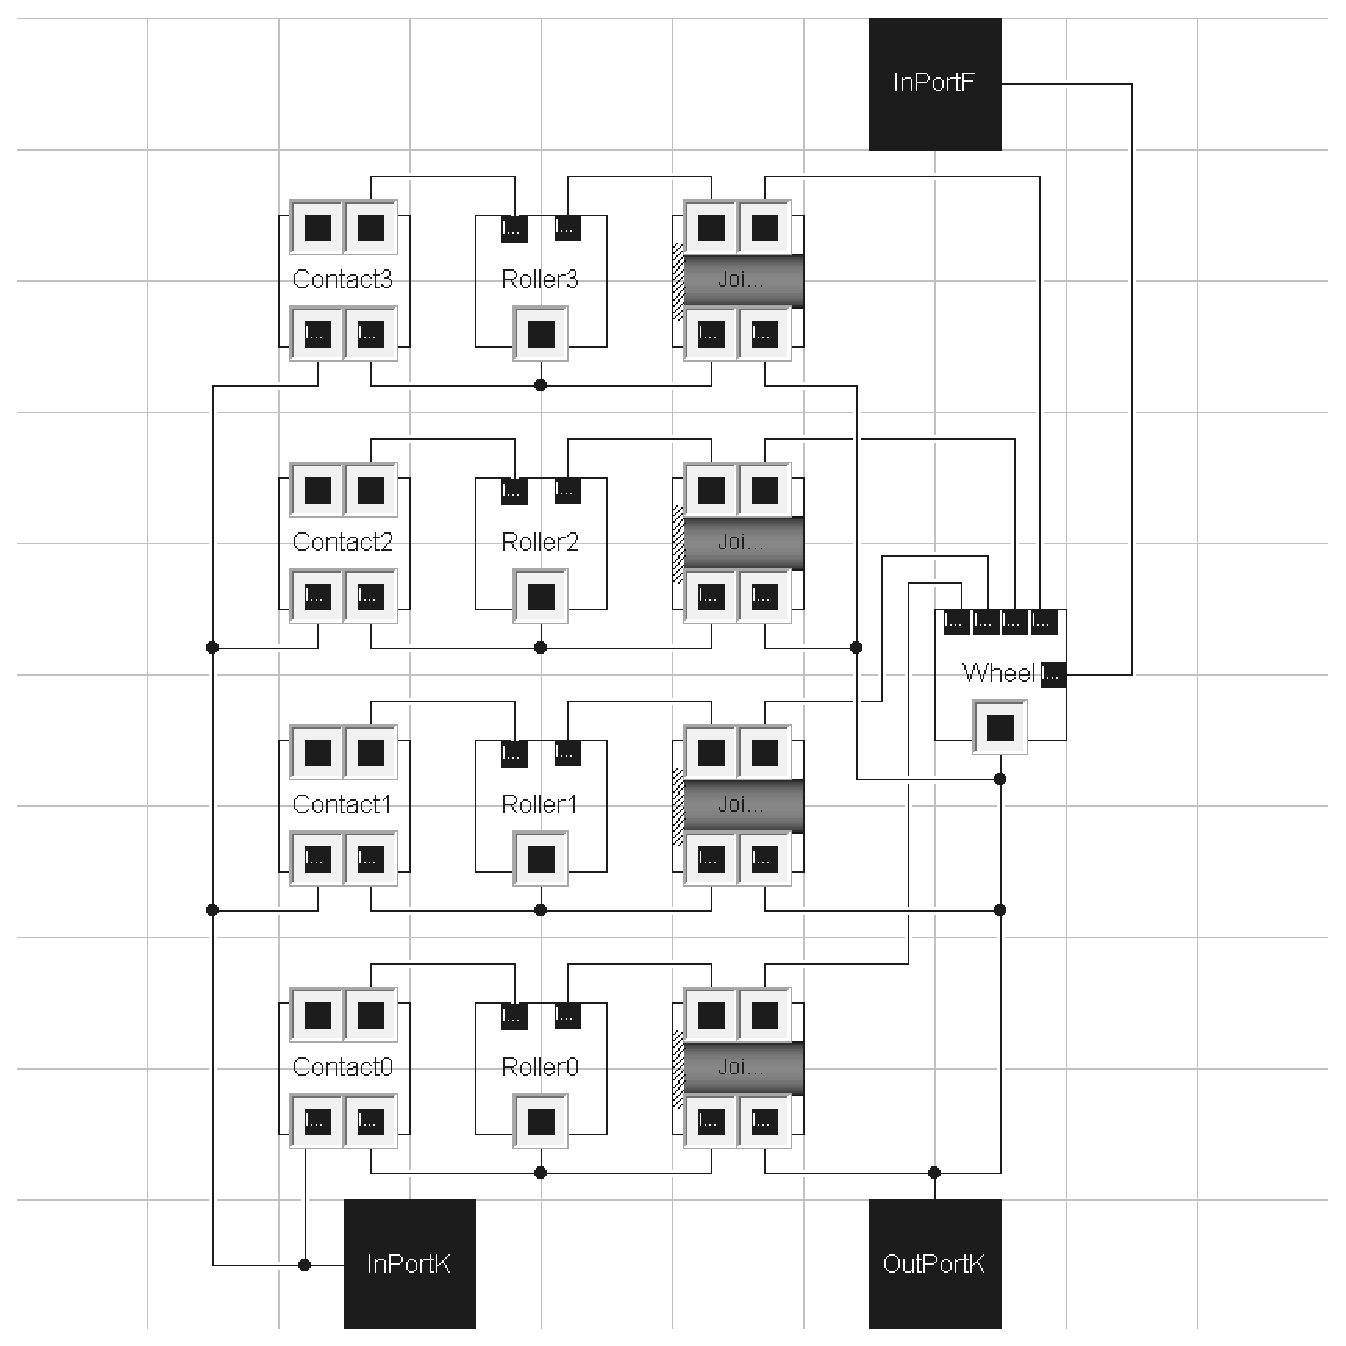
\includegraphics[width=15cm]{content/parts/3_friction/nd/OmniWheelModel.eps}
\caption{Визуальная модель омни--колеса.}
\label{OmniWheelModel}
\end{figure}

Для сборки $n$ роликов колеса (в нашем примере мы для определенности полагаем
$n=4$) мы использовали ранее развитую технику реализации шарнирных связей
различных типов~\cite{Kosenko2007}. В данном случае используется класс, 
задающий шарнир, обеспечивающий свободное относительное вращение одного тела
(ролика) относительно другого тела (колеса). Одновременно не допускается 
(поступательное) относительное перемещение тел вдоль оси шарнира. Визуальная 
модель омни--колеса изображена на Рис.~\ref{OmniWheelModel}. Дадим здесь более
подробное описание этой модели.

Вначале рассмотрим абстрактную схему информационных коммуникаций для одной,
отдельно взятой, механической связи. Эта схема показана на 
Рис.~\ref{ConstraintScheme}. Здесь $A$ и $B$ --- идентификаторы моделей двух 
твердых тел, взаимодействующих при помощи объекта связи. Общая схема такова: 
модели динамики тел $A$ и $B$, содержащие дифференциальные уравнения 
поступательно-вращательного движения в каждом экземпляре ($A$ и $B$) класса
<<Твердое тело>> при помощи численных интеграторов вырабатывает кинематическую
информацию о положении тел, их ориентации, скоростях и ускорениях. Вся эта 
информация у каждого из тел непрерывно поступает на экспорт из объектов $A$ и 
$B$ через соответствующий кинематический порт. У объекта тела имеется в 
точности один кинематический порт.

\begin{figure}[htb]
\centering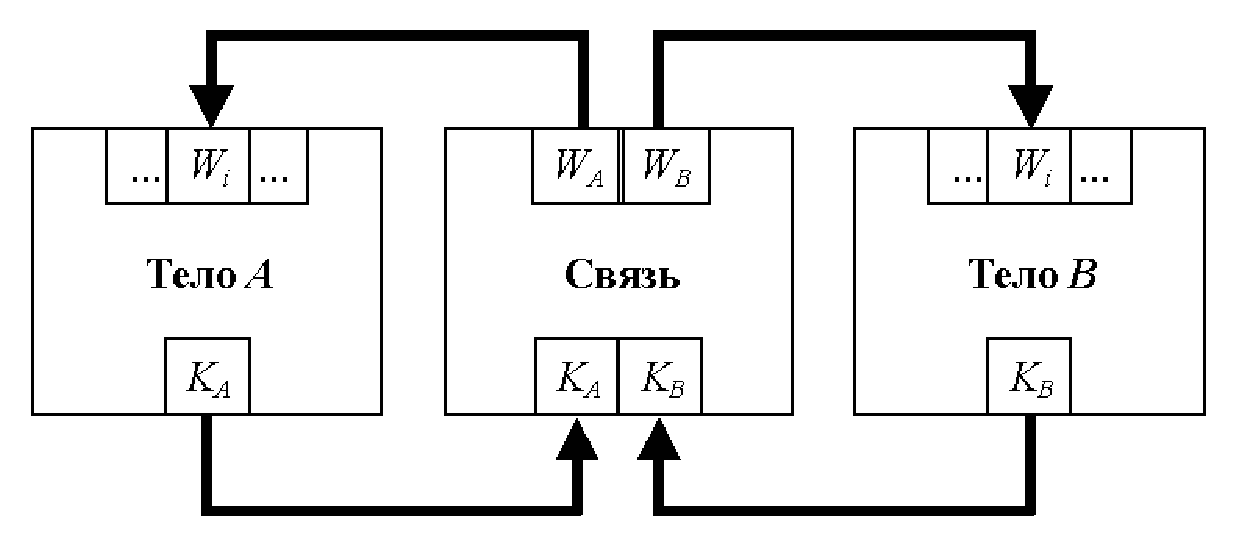
\includegraphics[width=14cm]{content/parts/3_friction/nd/Fig_2_1.eps}
\caption{Коммуникационная сеть механической связи.}
\label{ConstraintScheme}
\end{figure}

Кинематическую информацию от тел $A$ и $B$ также непрерывно во времени 
импортирует объект связи через два входных порта (Рис.~\ref{ConstraintScheme})
Внутри объекта связи эта информация (соответствующие переменные) 
<<пропускается>> через систему уравнений данного конкретного вида механической
связи. При этом объект связи <<вырабатывает>> и экспортирует через свои 
выходные силовые порты пары вида (<<сила>>, <<момент>>) = <<силовой мотор>>. 
Эта информация через два выходных порта поступает на вход в объекты $A$ и $B$.

Таким образом, коммуникационная сеть механической связи <<замыкается>>. Набор 
указанных пар взаимодействующих тел и составляет модель динамики систем тел. В
визуальных моделях омни-колеса и экипажа легко угадываются такие 
<<элементарные>> ячейки взаимодействия тел, на которые наложены механические 
ограничения (связи). Рассмотрим для определенности механическую систему 
омни-колеса (Рис.~\ref{OmniWheelModel}). Но сначала обратим внимание на 
визуальную модель экипажа (Рис.~\ref{OmniVehicle}). Здесь слева расположен 
объект базового тела --- горизонтального пола. Этот объект не имеет динамики.
Имеется только заданная кинематическая информация.

%\begin{figure}[ht]
%\centerline{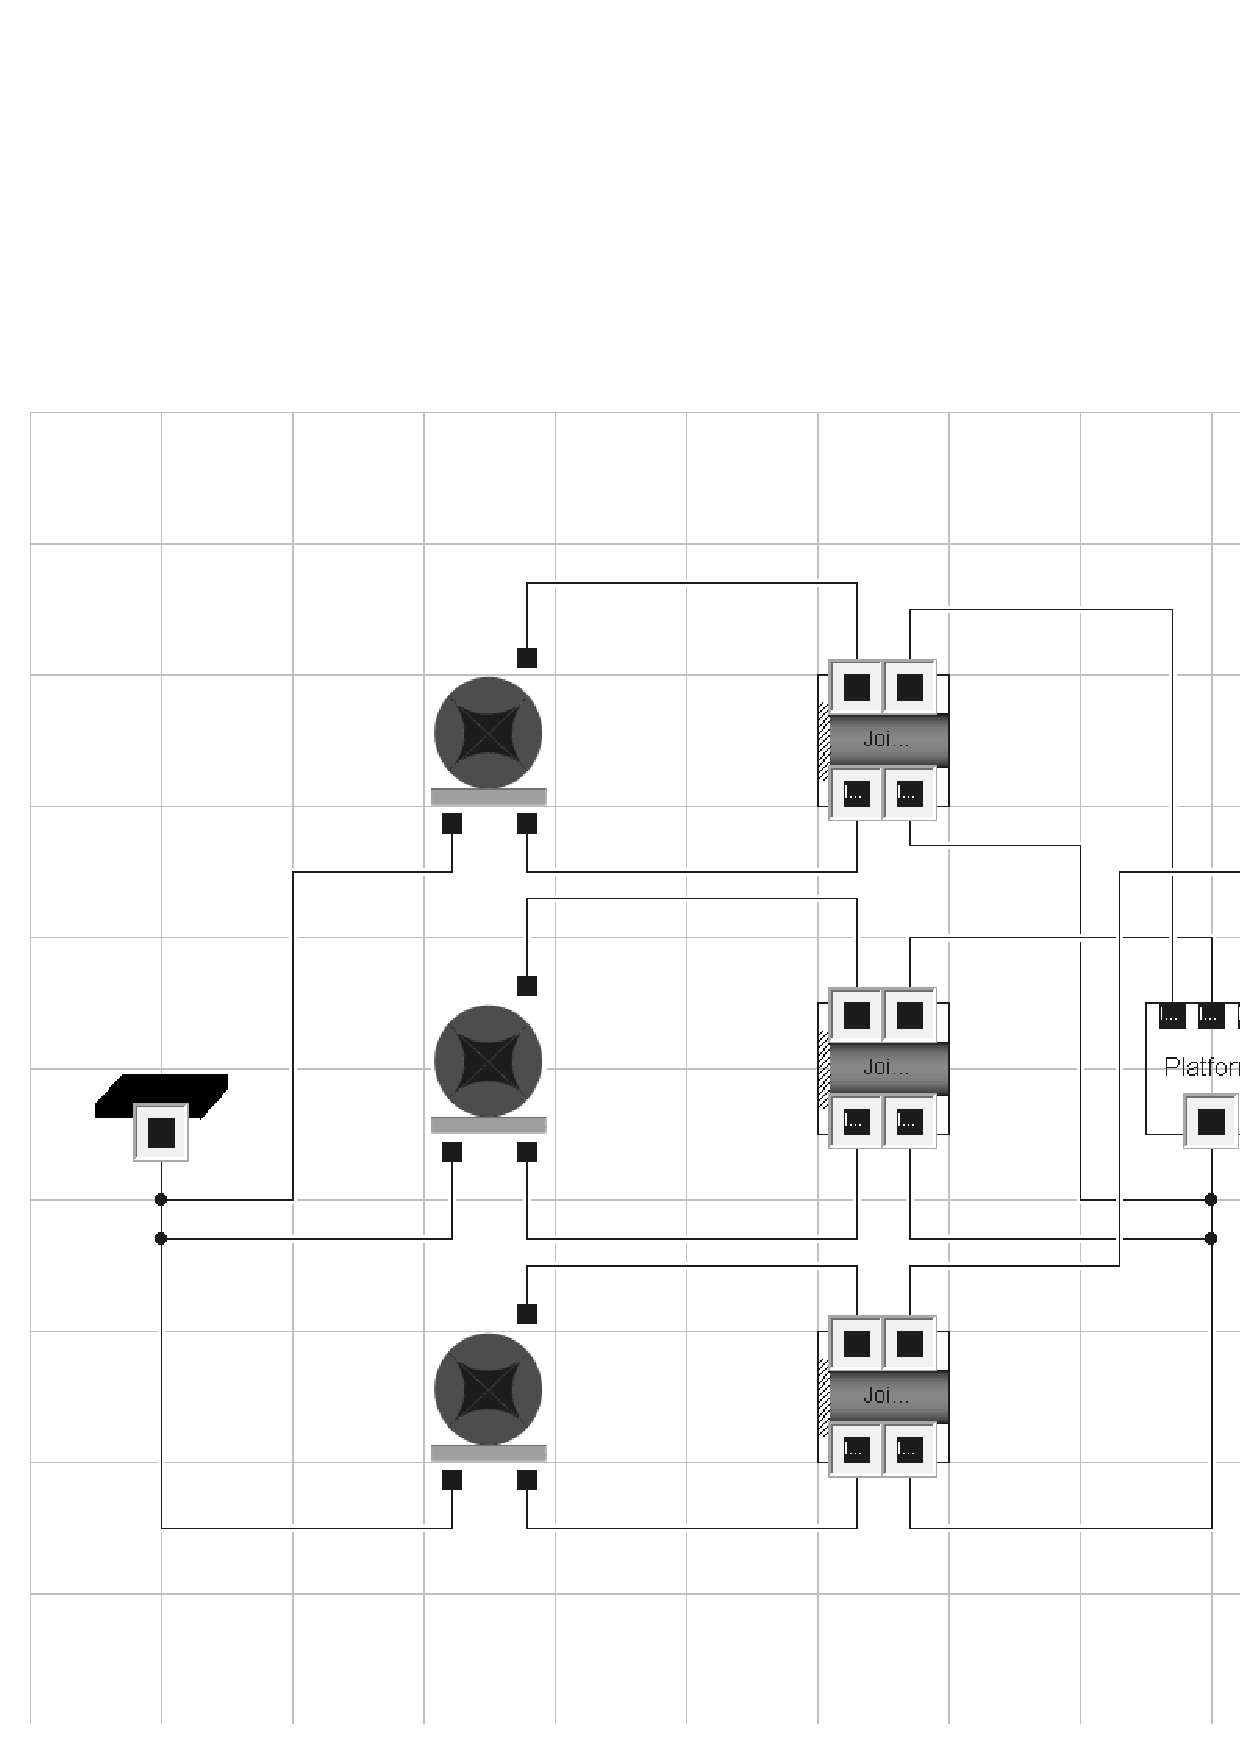
\includegraphics[bb= 0cm 0cm 20cm 20cm,scale=0.7]{OmniVehicleModel.png}}
%\caption{Визуальная модель омни--экипажа.}
%\label{OmniVehicle}
%\end{figure}
\begin{figure}[htb]
\centering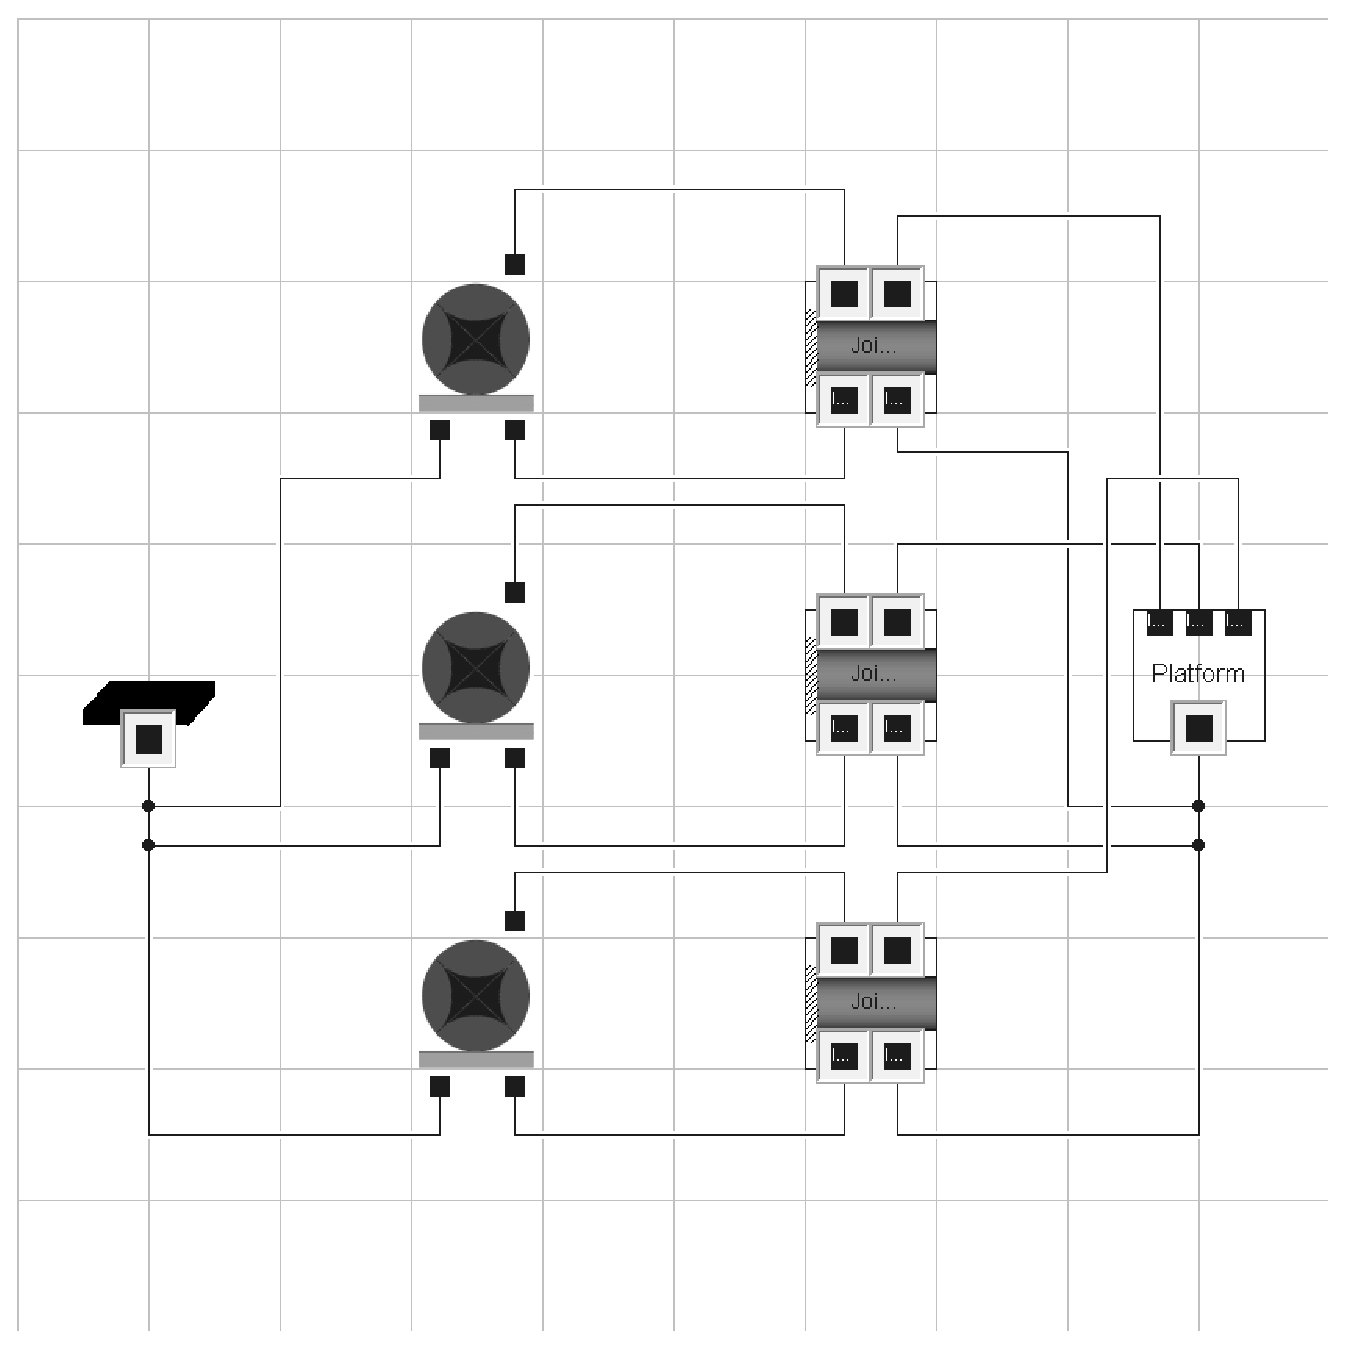
\includegraphics[width=15cm]{content/parts/3_friction/nd/OmniVehicleModel.eps}
\caption{Визуальная модель омни--экипажа.}
\label{OmniVehicle}
\end{figure}

Базовое тело и каждый из роликов омни-колеса находятся в контактном 
взаимодействии. Это взаимодействие реализуется при помощи порта $InPortK$
(Рис.~\ref{OmniWheelModel}), три экземпляра которого мы можем видеть на схеме
Рис.~\ref{OmniVehicle}. Здесь реализована неудерживающая связь, обеспечивающая 
в нашем конкретном случае точечный твердотельный контакт поверхности ролика и
поверхности пола. Причем, конструкция омни-колеса такова, что в каждый данный 
момент времени имеется имеется только один контакт. Остальные ролики <<висят>>
над полом. При этом механическая связь между полом и, <<висящим>> на ободе
колеса, роликом не исчезает --- алгоритм отслеживания контакта продолжает 
работать, генерируя в качестве реакций нулевые усилия и моменты.

В случае фактического выполнения контакта помимо нормальной реакции вычисляется
также её касательная составляющая, симулирующая силу трения. Для касательного 
контактного усилия имеется (как и для нормального) множество различных моделей. 
Мы остановились на реализации простейшего случая --- модели сухого трения при 
одноточечном твердотельном контакте. При этом, как известно~\cite{Novozhilov}, 
идеальный <<сухой>> случай реализовать не удается. Вместо разрывной функции 
sign от касательной скорости относительного скольжения контактирующих 
поверхностей используется её регуляризованный в нуле вариант. В нашем случае 
вместо функции знака sign применяется функция линейного насыщения, имеющая в 
окрестности нуля <<крутой>> линейный участок. Для таких функций известен 
результат~\cite{Novozhilov} о близости аппроксимирующего движения и движения, 
соответствующего <<точному>> случаю разрывной функции sign.

Обращаясь далее к визуальной модели омни-колеса, видим, что каждый из роликов 
соединен с ободом колеса при помощи цилиндрического шарнира (объекты связей
$Joint0,\dots ,Joint3$). Это модели шарниров, которые обеспечивают свободное
вращение роликов относительно корпуса колеса.

Кроме описанных объектов, составляющих модель динамики омни-колеса, эта модель
имеет порты своих внешних связей. Это уже упомянутый выше порт $InPortK$ связи
с базовым телом, а также порты $OutPortK$ (кинематика), $InPortF$ (усилия) 
соединений с шарнирами монтажа колес и корпуса всего экипажа (показаны на 
визуальной модели экипажа на Рис.~\ref{OmniVehicle}). Заметим здесь же, что 
каждый из объектов визуальной модели имеет набор соответствующих уравнений
(дифференциальных и/или алгебраических), порожденных из класса данного объекта.

В процессе отладки модели рассматривались автономные движения отдельного 
омни-колеса. Наибольший интерес представляет сборочный уровень всего экипажа
(Рис.~\ref{Vehicle}). Соединительные устройства были также реализованы как 
объекты того же самого шарнирного класса из шага а). Эти шарниры соединяют 
корпус экипажа и каждое из колес. Все упомянутые шарниры <<разрешают>> 
относительное вращение без какого-либо сопротивления и одновременно блокируют
скольжение вдоль оси шарнира. Визуальная модель экипажа показана на 
Рис~\ref{OmniVehicle}. Здесь для наглядности объекты показаны в виде скалярных
элементов. На самом деле при произвольном $n$ и произвольном числе и 
расположении колес следует использовать массивы объектов класса <<ролик>> и 
класса <<омни--колесо>>.

Заметим, что перед началом процесса редукции индекса системы 
дифференциально-алгебраических уравнений полной модели экипажа, реализованного
в программном обеспечении лаборатории динамического моделирования 
Dymola~\cite{Dymola}, эта модель составляется из: а) твердого тела платформы
омни--экипажа; б) трех твердых тел --- моделей омни--колес; в) двенадцати 
твердых тел роликов, размещенных на колесах. В соответствии, например, 
с~\cite{Kosenko2007} для каждого объекта, моделирующего твердое тело, 
реализуются шесть обыкновенных дифференциальных уравнений (ОДУ) Ньютона для
движения центра масс тела плюс семь ОДУ Эйлера для вращательного движения тела
вокруг центра масс. В последнем случае имеется четыре кинематических уравнения
Эйлера для кватерниона ориентации тела плюс три динамических уравнения Эйлера
для вектора угловой скорости твердого тела. В результате полная модель экипажа
задается системой ОДУ порядка $16\cdot 13=208$. Кроме этого, объекты 
механических связей могут генерировать дополнительные дифференциальные 
уравнения.

\begin{figure}[htb]
\centerline{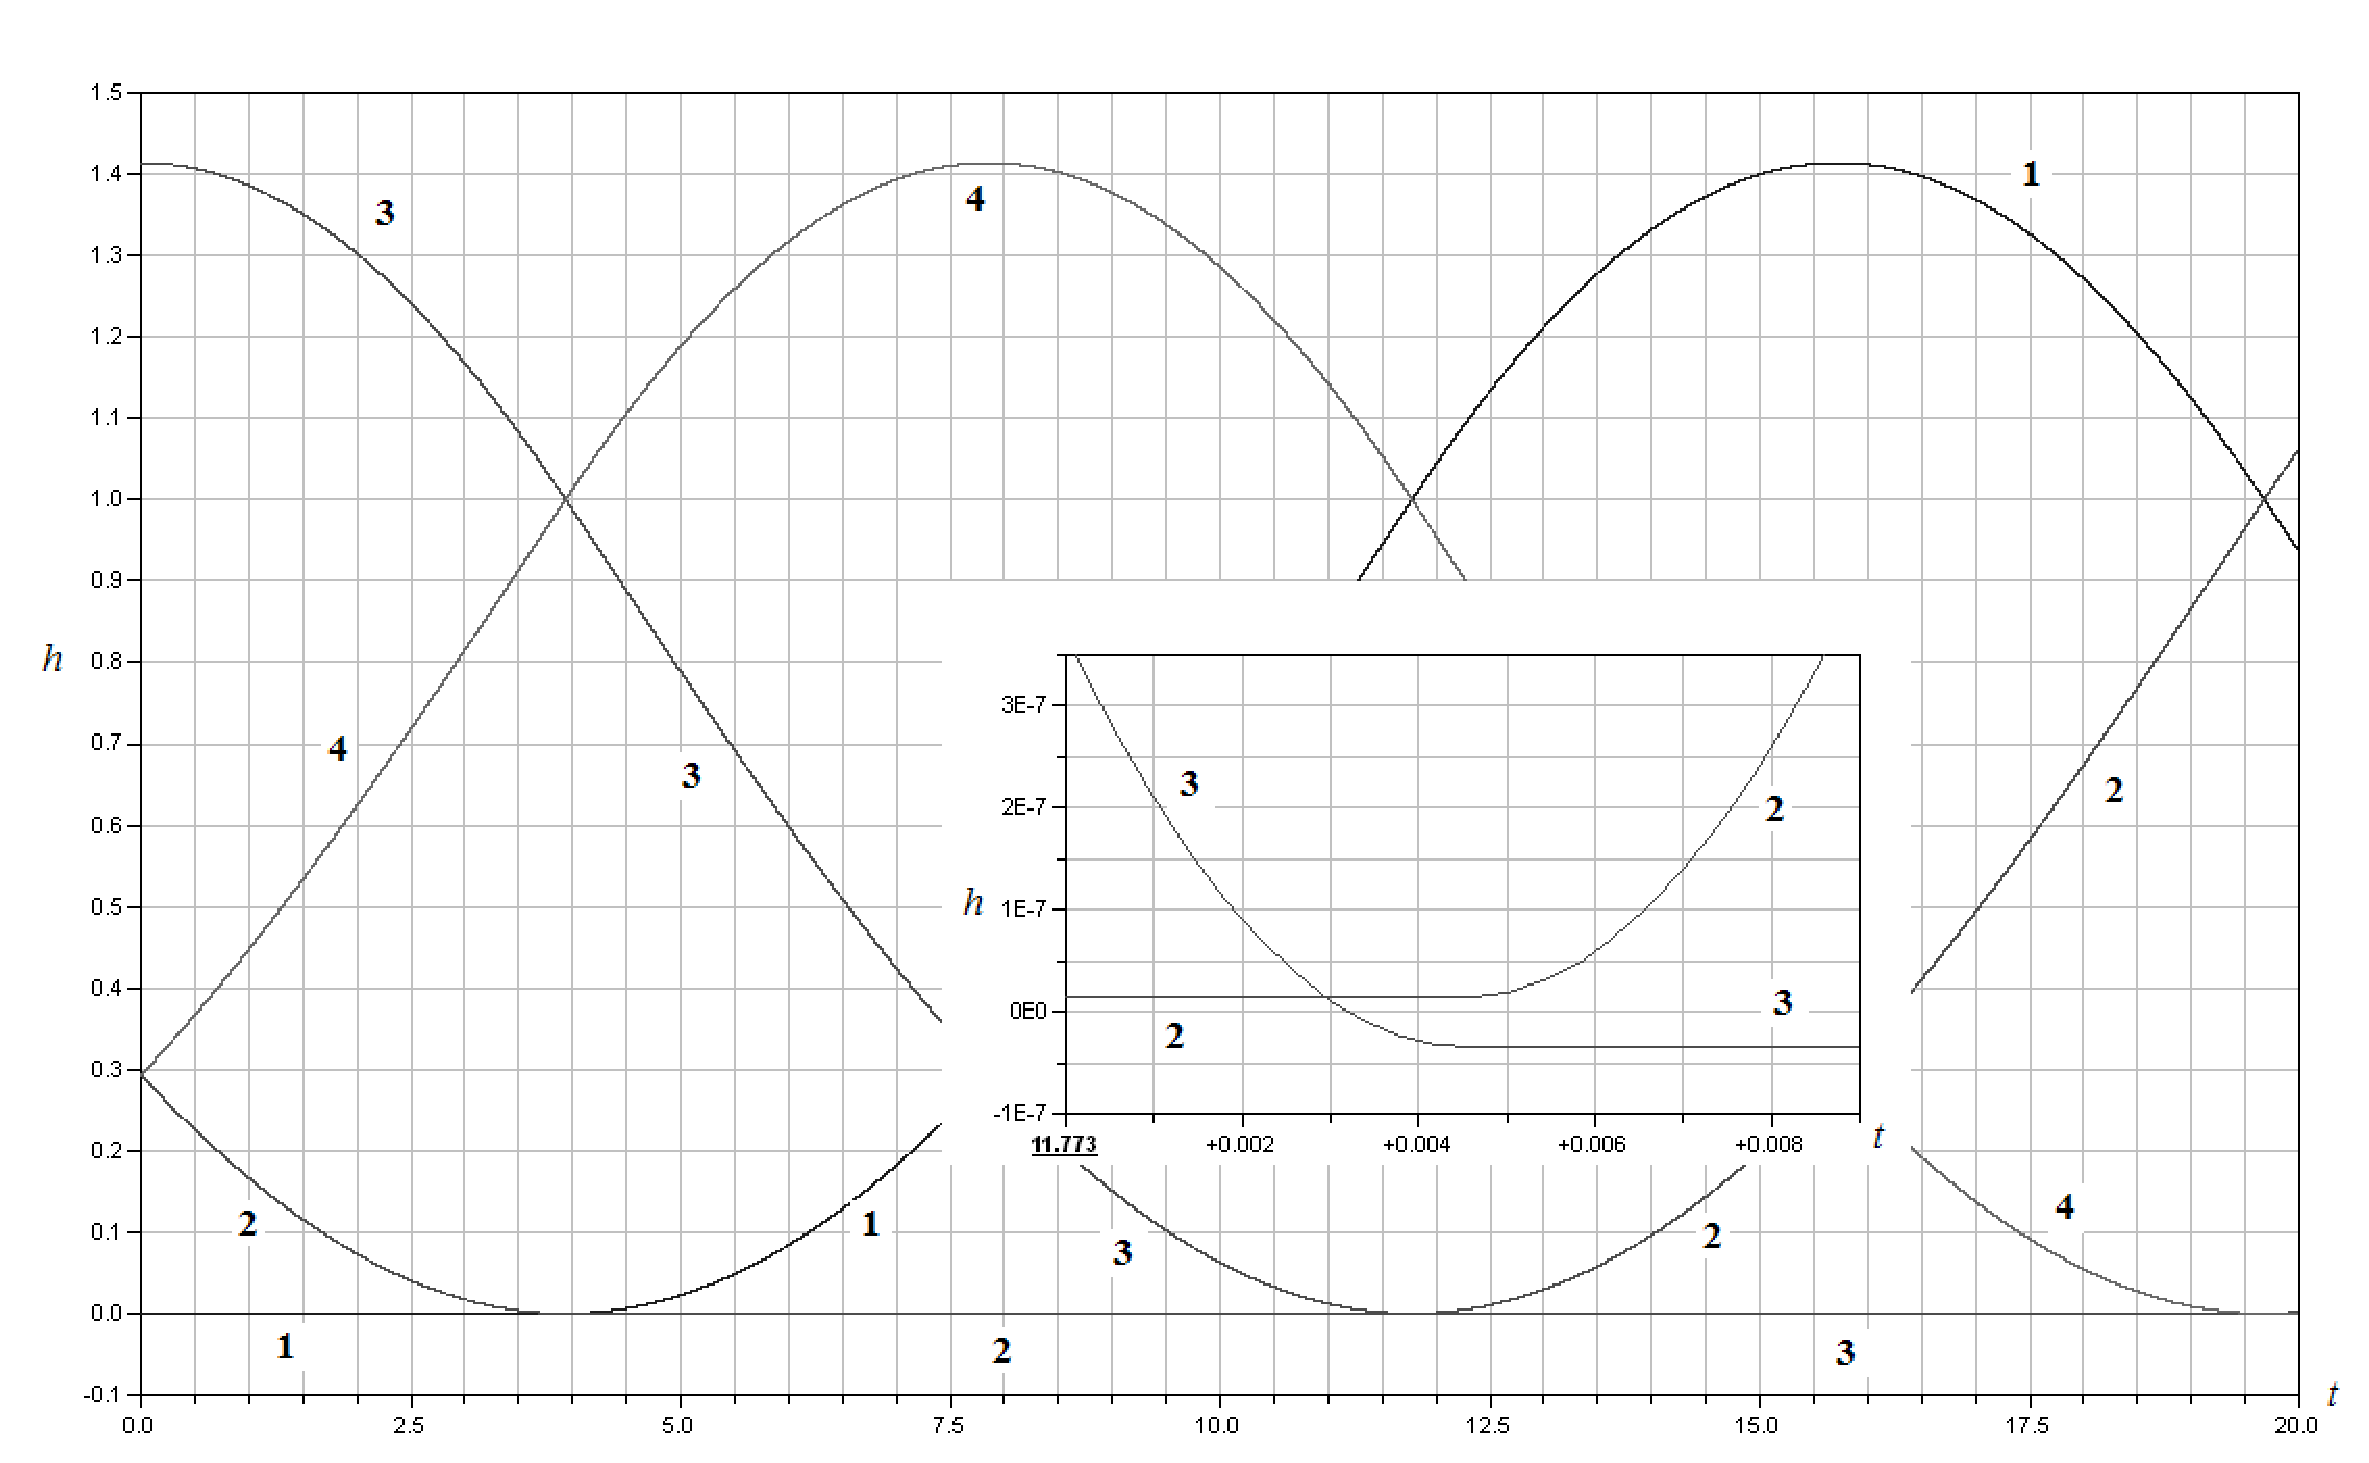
\includegraphics[width=15cm]{content/parts/3_friction/nd/Figure11.eps}}
\caption{Процесс замещения роликов в контакте.}
\label{fig1}
\end{figure}

Эволюция процесса контактирования для отдельного катящегося омни-колеса 
показана на Рис.~\ref{fig1}, где представлены зависимости функций расстояний 
$h$ (фактически --- высот) между горизонтальной плоскостью (полом) и роликами 
одного и того же колеса, находящимися в разных фазах (перед контактом, в 
контакте, после контакта). Функция высоты отдельного ролика помечена номером 
этого ролика. В увеличенном масштабе показан момент безударного гладкого 
переключения поверхностей контактирования роликов и горизонтальной плоскости.

Одновременно можно наблюдать точность соблюдения неудерживающей связи 
(Рис.~\ref{fig2}). Здесь обнаруживается процесс постепенного <<расползания>>
вычислительной ошибки --- расстояние между контактирующими телами медленно, для
каждого последующего ролика в контакте, увеличивается. В то же время, 
абсолютная величина ошибки остается пренебрежимо малой --- около $10^{-7}$
от единицы длины.

\begin{figure}[htb]
\centerline{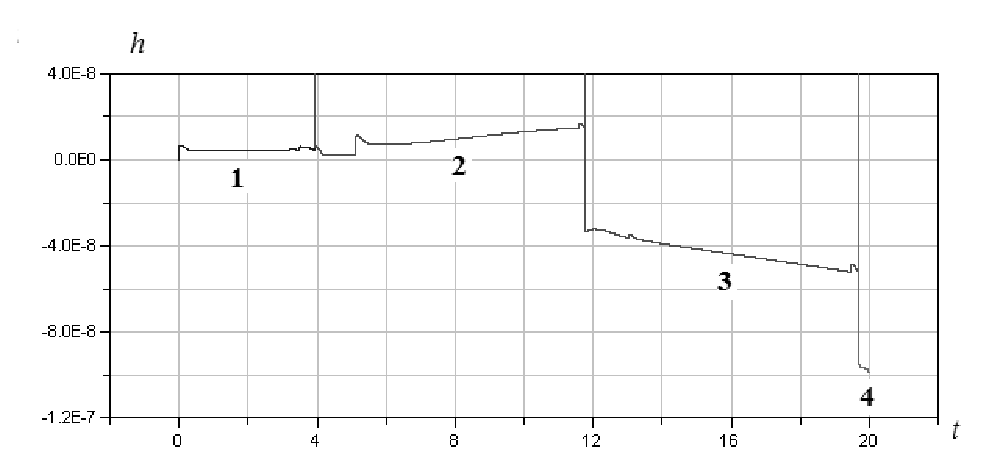
\includegraphics[width=15cm]{content/parts/3_friction/nd/Figure21.eps}}
\caption{Точность сохранения неудерживающей связи.}
\label{fig2}
\end{figure}
